\documentclass[12pt]{article}
\usepackage{amsmath}
\usepackage{arydshln}
\usepackage{hhline}
\usepackage{amsmath}
\usepackage{graphicx}
\usepackage{float}
\usepackage{chngcntr}
\usepackage[T1]{fontenc}
\usepackage[utf8]{inputenc}
\usepackage{subcaption}
\DeclareMathOperator{\sign}{sgn}
\usepackage{comment}
\usepackage{breqn}
\usepackage{bm}
\usepackage{tabularx,ragged2e,booktabs,caption}
\newcolumntype{C}[1]{>{\Centering}m{#1}}
\renewcommand\tabularxcolumn[1]{C{#1}}
\usepackage{mathtools}
\renewcommand{\arraystretch}{1.5}
\title{Car modelling}
\author{MarsvinTech}

\begin{document}
\maketitle

\section{System description}
\begin{figure}[H]
    \centering
    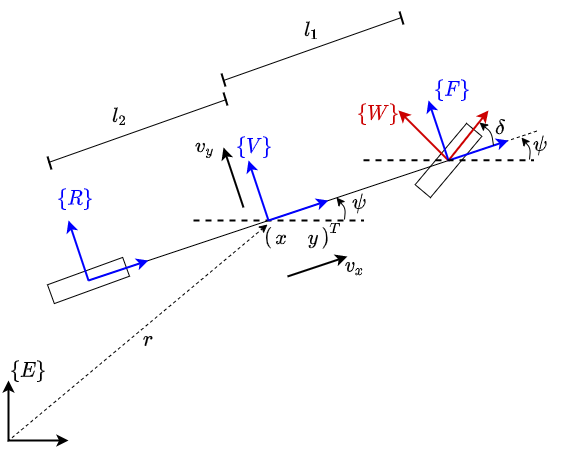
\includegraphics[scale=0.8]{images/car_modelling_1.png}
    \caption{Car model: Single axle bicycle model}
    \label{fig:car_system}
\end{figure}

\begin{figure}[H]
    \centering
    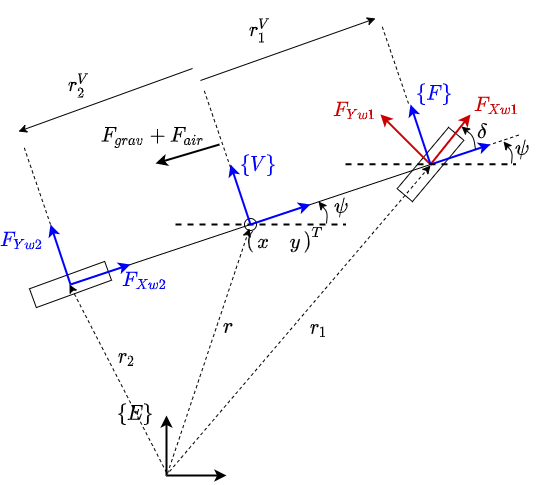
\includegraphics[scale=0.8]{images/car_modelling_forces.png}
    \caption{Car model: Position and forces vectors.}
    \label{fig:car_system_forces}
\end{figure}
\begin{table}[H]
\begin{tabular}{p{4cm} p{10cm}}
Frame $\{ E \}$& : Axis system fixed in the earth frame or reference frame.\\
Frame $\{ V \}$& : Axis system fixed in the center of gravity (CoG) of the car.\\
Frame $\{ W \}$& : Axis system fixed in the front wheel.\\
Frame $\{ F \}$& : Axis system fixed in the front axle (axle 1).\\
Frame $\{ R \}$& : Axis system fixed in the rear axle (axle 2).\\
$R^E_V$ & : Rotation matrix for Frame $\{ V \}$  (axis system fixed in the Cog of car) w.r.t. Frame $\{E\}$.\\
$R^E_W$ & : Rotation matrix for front wheel w.r.t. Frame $\{E\}$.\\
$r = \begin{pmatrix} x & y \end{pmatrix}^T$ & : Position vector of CoG of car w.r.t Frame $ \{ E \}$. Unit: $m$\\
$v = \dot{r} = \begin{pmatrix} \dot{x} & \dot{y} \end{pmatrix}^T$ & : Velocity vector of CoG of car w.r.t Frame $ \{ E \}$. Unit: $ \displaystyle \frac{m}{s}$\\
$v^V = \begin{pmatrix} v_x & v_y \end{pmatrix}^T$ & : Velocity vector of CoG of car w.r.t Frame $ \{ V \}$. Unit: $ \displaystyle \frac{m}{s}$\\
$a = \ddot{r} = \begin{pmatrix} \ddot{x} & \ddot{y} \end{pmatrix}^T$ & : Velocity vector of CoG of car w.r.t Frame $ \{ E \}$. Unit: $ \displaystyle \frac{m}{s^2}$\\
$r_1 = \begin{pmatrix} x_1 & y_1 \end{pmatrix}^T$ & : Position vector of axle 1 w.r.t Frame $ \{ E \}$. Unit: $m$\\
$v_1 = \dot{r}_1 = \begin{pmatrix} \dot{x}_1 & \dot{y}_1 \end{pmatrix}^T$ & : Velocity vector of axle 1 w.r.t Frame $ \{ E \}$. Unit: $ \displaystyle \frac{m}{s}$\\
$v^W_1 = \dot{r}_1 = \begin{pmatrix} v_{Xw1} & v_{Yw1} \end{pmatrix}^T$ & : Velocity vector of axle 1 w.r.t Frame $ \{ W \}$. Unit: $ \displaystyle \frac{m}{s}$\\
$r_2 = \begin{pmatrix} x_2 & y_2 \end{pmatrix}^T$ & : Position vector of axle 2 w.r.t Frame $ \{ E \}$. Unit: [m]\\
$v_2 = \dot{r} = \begin{pmatrix} \dot{x}_2 & \dot{y}_2 \end{pmatrix}^T$ & : Velocity vector of axle 2 w.r.t Frame $ \{ E \}$. Unit: $ \displaystyle \frac{m}{s}$\\
$v^V_2 = \begin{pmatrix} v_{Xw2} & v_{Yw2} \end{pmatrix}^T$ & : Velocity vector of axle 2 w.r.t Frame $ \{ E \}$. Unit: $ \displaystyle \frac{m}{s}$\\
$\psi$  & : Inclination of Unit 1 w.r.t x-axis of Frame $ \{ E \}$. Unit: rad\\
$\delta$  & : Wheel steer angle of front wheel w.r.t x-axis of Frame $ \{ E \}$. Unit: rad\\
\end{tabular}
\end{table}

\begin{table}[H]
\begin{tabular}{p{4cm} p{10cm}}
$l_1$ & : Distance between axle 1 (front axle) and centre of gravity. Unit: $m$\\
$l_2$ & : Distance between axle 2 (rear axle) and centre of gravity. Unit: $m$\\
$C_{y1}$ & : Cornering stiffness axle 1. Unit: $\frac{N}{rad}$\\
$C_{y2}$ & : Cornering stiffness axle 2. Unit: $\frac{N}{rad}$\\
$m$ & : Car mass. Unit: $Kg$\\
$J$ & : Inertia around z-axis of vehicle Unit. Unit: $kg.m^2$\\
%$( X_E, Y_E )$ & : Axis system fixed in the earth frame (Frame $ \{ E \}$);\\
%$( X_{W11}, Y_{W11} )$ & : Axis system fixed in unit 1 axle 1 (Frame $ \{ W \}$);\\
%$( X_{V1}, Y_{V1} )$ & : Axis system fixed in unit 1 (Frame $ \{ 1 \}$);\\
%$( X_{V2}, Y_{V2} )$ & : Axis system fixed in unit 2 (Frame $ \{ 2 \}$).\\
\end{tabular}
\end{table}

\section{Rotation matrices}
The following rotation matrices of Frame $\{ V \}$ and $\{ W \}$ with respect to Frame $\{ E \}$ are calculated by,

\begin{equation}
    R_{V}^E = R_{F}^E =R_{R}^E =R_z (\psi) = \begin{pmatrix} \cos{\psi} & - \sin{\psi} \\ \sin{\psi} & \cos{\psi} \end{pmatrix}
\end{equation}

\begin{equation}
    R_{W}^E = R_z (\psi + \delta) = \begin{pmatrix} \cos{(\psi + \delta)} & - \sin{(\psi + \delta)} \\ \sin{(\psi + \delta)} & \cos{(\psi + \delta)} \end{pmatrix}
\end{equation}

Additionally, we can calculate the rotation matrix of Frame $\{ W \}$ with respect to Frame $\{ E \}$ by, 
\begin{equation}
    R_{W}^V =R_z (\delta) = \begin{pmatrix} \cos{\delta} & - \sin{\delta} \\ \sin{\delta} & \cos{\delta} \end{pmatrix}
\end{equation}

Some properties for rotation matrices,
\begin{equation}
R^{-1} = R^T    
\end{equation}
\begin{equation}
R^{n}_{p} = R^{n}_m R^{m}_p     
\end{equation}
\begin{equation}
    r^n = R^n_p r^p
\end{equation}
where $r^i$ is the vector $r$ represented in the Frame ${i}$ and $R^i_j$ is the rotation matrix of Frame $\{ j \}$ with respect to Frame $\{ i \}$.
\section{Car dynamics using Euler-Lagrange equation}
Some manipulations were done using the Euler-Lagrange equation in order to obtain the state-space equation. This steps are a bit different than other steps published in some articles and books. These steps help to compute the differential equation use for the state-space expression.

The Euler-Lagrange equation is defined by,
\begin{equation}
    \frac{d}{dt} \Big( \frac{\partial \mathcal{L}(q,\dot{q})}{\partial \dot{q}} \Big) - \frac{\partial \mathcal{L}(q,\dot{q})}{\partial q} = Q
\end{equation}
where $q$ is the generalized coordinates, $\mathcal{L} (q,\dot{q})$ is the Lagrangian and $Q$ are the generalized forces of the system.

The Lagrangian is defined as,
\begin{equation}
\mathcal{L} (q,\dot{q}) = T(q,\dot{q}) - V(q)    
\end{equation}
where $T$ is the kinetic energy and $V$ is the potential energy. For car modeling, the potential energy can be neglected, therefore the Euler-Lagrange equation can be expressed as,

\begin{equation} \label{eq_el_1}
    \frac{d}{dt} \Big( \frac{\partial T(q,\dot{q}) }{\partial \dot{q}} \Big) - \frac{\partial T(q,\dot{q}) }{\partial q} = Q
\end{equation}

Then by using chain-rule, the following equivalent expressions can be obtained,

\begin{equation} \label{eq_el_2}
  \frac{d}{dt} \Big( \frac{\partial T(q,\dot{q}) }{\partial \dot{q}} \Big) = \frac{\partial }{\partial q} \Big( \frac{\partial T(q,\dot{q})}{\partial \dot{q}} \Big) \dot{q} + \frac{\partial }{\partial \dot{q}} \Big( \frac{\partial T(q,\dot{q})}{\partial \dot{q}} \Big) \ddot{q}  
\end{equation}
using \eqref{eq_el_2} in \eqref{eq_el_1} and solving for $\ddot{q}$,
\begin{equation}
    \ddot{q} =  \Bigg(  \frac{\partial }{\partial \dot{q}} \Big( \frac{\partial T(q,\dot{q})}{\partial \dot{q}} \Big) \Bigg)^{-1} \Bigg( \frac{ \partial T(q,\dot{q})}{\partial q} - \frac{\partial }{\partial q} \Big( \frac{\partial T(q,\dot{q})}{\partial \dot{q}} \Big) \dot{q} + Q \Bigg)
\end{equation}
\subsection{Generalized coordinates}
\begin{equation} \label{Generalized_coordinates_eq}
    q = \begin{pmatrix} x \\ y \\ \psi \end{pmatrix} \quad \longrightarrow \quad \dot{q} = \begin{pmatrix} \dot{x} \\ \dot{y} \\ \dot{\psi} \end{pmatrix} \quad \longrightarrow \quad \ddot{q} = \begin{pmatrix} \ddot{x} \\ \ddot{y} \\ \ddot{\psi} \end{pmatrix}
\end{equation}
\subsection{Kinetic energy}
The total kinetic energy for the semi-trailer combination is given by,
\begin{equation}
    T(q,\dot{q}) = \frac{1}{2}m \dot{r}^T \dot{r}  + \frac{1}{2}J\dot{\psi}^2
\end{equation}
using chain rule, $\dot{r}$ can be calculated by,
\begin{equation}
    \dot{r} = \frac{\partial r}{\partial q}\dot{q}
\end{equation}

\subsection{Generalized forces}
The generalized forces can be calculated by,
\begin{equation}
    Q =  \Big( \frac{\partial r}{\partial q} \Big)^T F + \Big( \frac{\partial r_{1}}{\partial q} \Big)^T F_{1} + \Big( \frac{\partial r_{2}}{\partial q} \Big)^T F_{2}
\end{equation}
where $F$ is the force applied on the center of gravity of the car and $F_j$ is the force applied on axle $j$. All of these forces are represented in Frame $\{ E \}$.

In this case, we will neglected the forces by gravity (roads with slope) or aerodynamics (air) on the car. Therefore,

\begin{equation}
    F = - F_{grav} - F_{air} = 0
\end{equation}

In order to calculate $r_j$, were $j$ is the axle number, we can define the position vector of each axle in Frame $\{ V \}$,

\begin{equation}
    r_1^V = \begin{pmatrix} l_1 \\ 0 \end{pmatrix}
\end{equation}

\begin{equation}
    r_2^V = \begin{pmatrix} - l_2 \\ 0 \end{pmatrix}
\end{equation}

Then, the position vector of each axle in Frame {E} can be calculated by,

\begin{equation}
    r_1 = r_1^E =r + R^E_V r^V_1     
\end{equation}

\begin{equation}
    r_2 = r_2^E = r+ R^E_V r^V_2
\end{equation}

The forces applied on each tyre (or wheel) with respect to the corresponding tyre frame can be calculated by,

\begin{equation}
    F_1^W =  \begin{pmatrix} F_{Xw1} \\ F_{Yw1} \end{pmatrix}  = \begin{pmatrix}  F_{prop,1} + F_{brake,1} \\  - C_{Y1} \frac{v_{Yw1}}{v_{Xw1}}\end{pmatrix} 
\end{equation}

\begin{equation}
    F_2^R = \begin{pmatrix} F_{Xw2} \\ F_{Yw2} \end{pmatrix} = \begin{pmatrix} F_{prop,2} + F_{brake,2} \\  - C_{Y2} \frac{v_{Yw2}}{v_{Xw2}}\end{pmatrix}
\end{equation}
where $F_{prop,j}$ is the propulsion force on tyre $j$, $F_{brake,j}$ the braking force on tyre $j$, $C_{Yj}$ is the cornering stiffness of tyre $j$ and $\begin{pmatrix} v_{Xwj} & v_{Ywj} \end{pmatrix}^T$ is the velocity vector of tyre $j$ with respect to the frame fixed to the tyre.

Those values are obtained using,
\begin{equation}
    \begin{pmatrix} v_{Xw1} \\ v_{Yw1} \end{pmatrix} = R^W_E \dot{r}_1
\end{equation}
\begin{equation}
    \begin{pmatrix} v_{Xw2} \\ v_{Yw2} \end{pmatrix} = R^R_E \dot{r}_2
\end{equation}
where,
\begin{equation}
    \dot{r}_1 = \frac{\partial r_1}{\partial q} \dot{q}
\end{equation}

\begin{equation}
    \dot{r}_2 = \frac{\partial r_2}{\partial q} \dot{q}
\end{equation}

Additionally, it is assumed that propulsion and braking is only applied in tyre 2. Then,
\begin{equation}
    F_{prop,1} = F_{brake,1} = 0
\end{equation}

Forces applied on each tyre can be obtained by,

\begin{equation}
    F_1 = R^E_W F_1^W
\end{equation}
\begin{equation}
    F_2 = R^E_R F_2^R
\end{equation}

After all the operations, $\ddot{q}$ is estimated as a function of $\psi$, $\dot{x}$, $\dot{y}$ and $\dot{\psi}$,

\begin{equation}
    \ddot{q} = \begin{pmatrix} \ddot{x} \\ \ddot{y} \\ \ddot{\psi} \end{pmatrix} = \mathcal{F} (\psi,\dot{x},\dot{y},\dot{\psi})
\end{equation}

Since the velocity sensors on the car measure the longitudinal and lateral velocity of the car with respect of Frame $\{ V \}$. So we want something like,

\begin{equation}
    \ddot{q}_v = \begin{pmatrix} \dot{v}_x \\ \dot{v}_y \\ \ddot{\psi} \end{pmatrix} = \mathcal{F}(\psi,v_x,v_y,\dot{\psi})
\end{equation}
then we should transform,
\begin{equation} \label{eq_vel_rotation}
    \begin{pmatrix} \dot{x} \\ \dot{y} \end{pmatrix} = R^E_V \begin{pmatrix} v_x \\ v_y \end{pmatrix}  = \begin{pmatrix} v_x \cos{\psi} - v_y \sin{\psi} \\ v_x \sin{\psi} + v_y \cos{\psi}  \end{pmatrix}
\end{equation}

Moreover, calculating the derivative with respect to time of \eqref{eq_vel_rotation},

\begin{equation}\label{Rot_eq_derivative}
    \begin{pmatrix} \ddot{x} \\ \ddot{y} \end{pmatrix} = \dot{R}^E_{V} \begin{pmatrix} v_{x} \\ v_{y} \end{pmatrix} + R^E_{V} \begin{pmatrix} \dot{v}_{x} \\ \dot{v}_{y} \end{pmatrix}
\end{equation}
Rewriting \eqref{Rot_eq_derivative},
\begin{equation}\label{velocity_fixed_unit_1_eq}
    \begin{pmatrix} \dot{v}_{x} \\ \dot{v}_{y} \end{pmatrix} = R^V_{E}  \begin{pmatrix} \ddot{x} \\ \ddot{y} \end{pmatrix} - R^V_{E} \dot{R}^E_{V} \begin{pmatrix} v_{x} \\ v_{y} \end{pmatrix} 
\end{equation}

\section{State-space model}

\subsection{Nonlinear state-space model: Lateral and longitudinal dynamics}
The following state and input vectors are selected for the semi-trailer nonlinear model,
\begin{equation}\label{NL_states_input}
    \mathcal{X}_{NL} = \begin{pmatrix} v_{x} \\ v_{y} \\ \Dot{\psi} \end{pmatrix} \quad , \quad U_{NL} = \begin{pmatrix} \delta \\ F_{Xw2} \end{pmatrix}
\end{equation}
The nonlinear state-space model is defined by,
\begin{equation}
	\label{Nonlinear_state_space_eq}
    \Dot{\mathcal{X}}_{NL} = \begin{pmatrix} \Dot{v}_{x1}  \\ \Dot{v}_{y1} \\ \Ddot{\psi}_1 \end{pmatrix} = f_{NL}(\mathcal{X}_{NL},U_{NL})
\end{equation}

\subsection{Nonlinear state-space model: Only lateral dynamics }
In order to consider only lateral dynamics, it is possible to assume constant longitudinal velocity,
\begin{equation}
    v_x = \mathrm{Constant}
\end{equation}
For constant longitudinal velocity, it is assumed that the sum of the projections to $x$-axis of Frame $\{ V \}$ of all the forces apply to the car is zero, i.e.,
\begin{equation}
    F_{Xw1} \cos{\delta} - F_{Yw1} \sin{\delta} + F_{Xw2} = 0
\end{equation}
The following state and input vectors are selected for the semi-trailer nonlinear model,
\begin{equation}\label{NL_states_input_vx}
    \mathcal{X}_{nl} = \begin{pmatrix} v_{y} \\ \Dot{\psi} \end{pmatrix} \quad , \quad U_{nl} = \delta 
\end{equation}
The nonlinear state-space model is defined by,
\begin{equation} \label{Nonlinear_state_space_vx_eq}
    \Dot{\mathcal{X}}_{nl} = \begin{pmatrix} \Dot{v}_{y1} \\ \Ddot{\psi}_1 \end{pmatrix} = f_{nl}(\mathcal{X}_{nl},U_{nl})
\end{equation}

\subsection{Linear state-space model: Lateral and longitudinal dynamics}

In order to linearize $f_{NL}$ (showed in \eqref{Nonlinear_state_space_eq}), the following equilibrium $ \begin{pmatrix} \mathcal{X}_e & \mathcal{Y}_e\end{pmatrix}^T$ point is selected,

\begin{equation}
    \mathcal{X}_e = \begin{pmatrix} v_{xe} \\ v_{ye} \\ \Dot{\psi}_{e} \end{pmatrix} = \begin{pmatrix} v_{xd} \\ 0 \\ 0  \end{pmatrix} \quad , \quad U_e = \begin{pmatrix} \delta_{e} \\ F_{Xw2e} \end{pmatrix} = \begin{pmatrix} 0 \\ 0 \end{pmatrix}
\end{equation}

where $v_{xd}$ is the desired longitudinal velocity of the car. Additionally, around the equilibrium point no acceleration or braking is needed in order to keep constant longitudinal velocity. Therefore, $F_{Xw2e}$ can be approximated to zero,

\begin{equation}
    F_{Xw2e} = 0
\end{equation}

Then, $f_{NL}$ can be linearized around the equilibrium point ($\mathcal{X}_e$,$U_e$),

\begin{equation} \label{linear_expression_state}
    \dot{\mathcal{X}} = f_{LINEAR} = A (v_{xd}) \mathcal{X} + B (v_{xd}) U
\end{equation}

\subsection{Linear state-space model: Lateral dynamics}
In order to linearize $f_{nl}$ (showed in \eqref{Nonlinear_state_space_vx_eq}), the following equilibrium $ \begin{pmatrix} \mathcal{X}_e & \mathcal{Y}_e\end{pmatrix}^T$ point is selected,

\begin{equation}
    \mathcal{X}_e = \begin{pmatrix} v_{ye} \\ \Dot{\psi}_{e} \end{pmatrix} = \begin{pmatrix} 0 \\ 0  \end{pmatrix} \quad , \quad U_e =  \delta_{e} =  0 
\end{equation}

Then, $f_{nl}$ can be linearized around the equilibrium point ($\mathcal{X}_e$,$U_e$),

\begin{equation} \label{linear_expression_state}
    \dot{\mathcal{X}} = f_{linear} = A (v_{xd}) \mathcal{X} + B (v_{xd}) U
\end{equation}

\end{document}
